\begin{figure}[t]
\centering
\begin{tabular}{c}
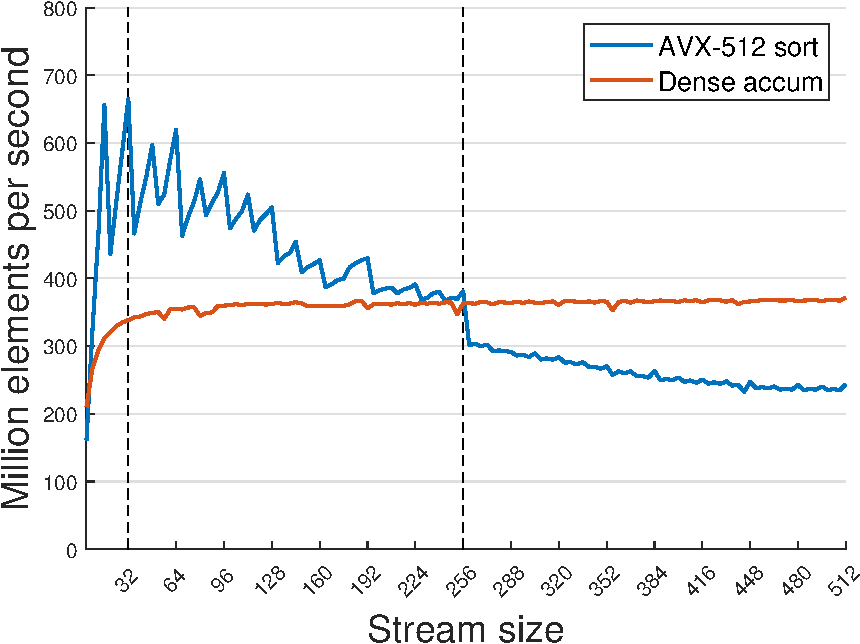
\includegraphics[width=\figwidth]{figs/sort_benchmark_sortSize.pdf}
\end{tabular}
\caption{Comparison of accumulators used in MAGNUS: AVX-512 vectorized sorting and dense accumulation.
A single core of the SPR system is used (see \autoref{tab:machines}).
The rate (millions of elements per second) versus the number of accumulated elements is shown.
The dashed lines indicate where the sorting achieves peak performance (32 elements) and where the performance of dense accumulation overtakes that of sorting (256 elements).}
\label{fig:sort_benchmark}
\end{figure}


\section{Experimental Results}\label{sec:results}

\subsection{Microbenchmarks}\label{sec:microbench}
This section aims to establish our motivation by evaluating the core building blocks of MAGNUS in isolation through microbenchmarking.
The input and output in our microbenchmarks are streams consisting of two arrays of the same size: one of unsigned integers (the \textit{index array}) and the other of floating-point numbers (the \textit{value array}), which emulate the column indices and values, respectively, in the intermediate product.
There are two critical parameters to which SpGEMM accumulators are sensitive: the number of elements in the stream and the maximum value of the elements in the index array (the \textit{stream length}).
The index array is uniformly random in the range $[0, \text{stream length})$, which emulates the range of column indices in the matrix or a MAGNUS chunk.

First, we show that increasing the stream size and length degrades the performance of conventional accumulators.
We then benchmark the building blocks of MAGNUS to demonstrate how the introduction of locality generation can improve the performance of the dense accumulator.
For these experiments, four-byte types were used (\texttt{uint32\_t} and \texttt{float}) on one core of the SPR system (see \autoref{tab:machines}).
We used Likwid~\cite{likwid} to collect performance metrics, providing insight into the cache behavior of the building blocks of MAGNUS.
Likwid is a performance monitoring tool that reports detailed CPU hardware metrics, including the volume of L2-to-L3 cache evictions.

\subsubsection{Accumulators}\label{sec:results_sort}
We first consider the two accumulators used by MAGNUS: AVX-512 vectorized bitonic sorting~\cite{AVX512sort} and dense accumulation.
\autoref{fig:sort_benchmark} shows the rate (in millions of elements per second) versus the stream size for a fixed stream length of $2^{18}$, which is the stream length for which the dense accumulation arrays fit into the L2 cache.
There are two important sizes to consider: 32 and 256. At a size of 32, the sorting achieves peak performance, processing nearly 700 million elements per second. Therefore, targeting sort sizes as close as possible to 32 is ideal.
In MAGNUS, we do precisely this: we combine consecutive chunks until the difference between the sort size and 32 is minimized.
Dense accumulation overtakes sorting at a stream size of 256 and is $\approx 1.5\times$ faster for a sort size of 512.
The 256 threshold originates from the sorting algorithm, which partitions the array into 256 parts (for more information, see~\cite{AVX512sort}).
MAGNUS uses this threshold when selecting an accumulator within a chunk.

\begin{figure}[t]
\centering
\begin{tabular}{c}
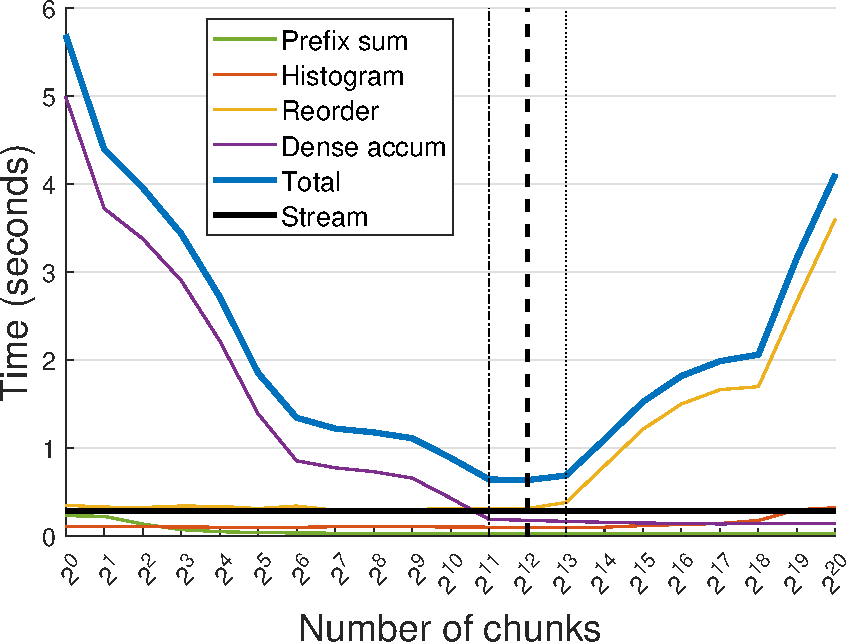
\includegraphics[width=\figwidth]{figs/spr_buildingBlocks_varyChunks_scale29_time.pdf} \\
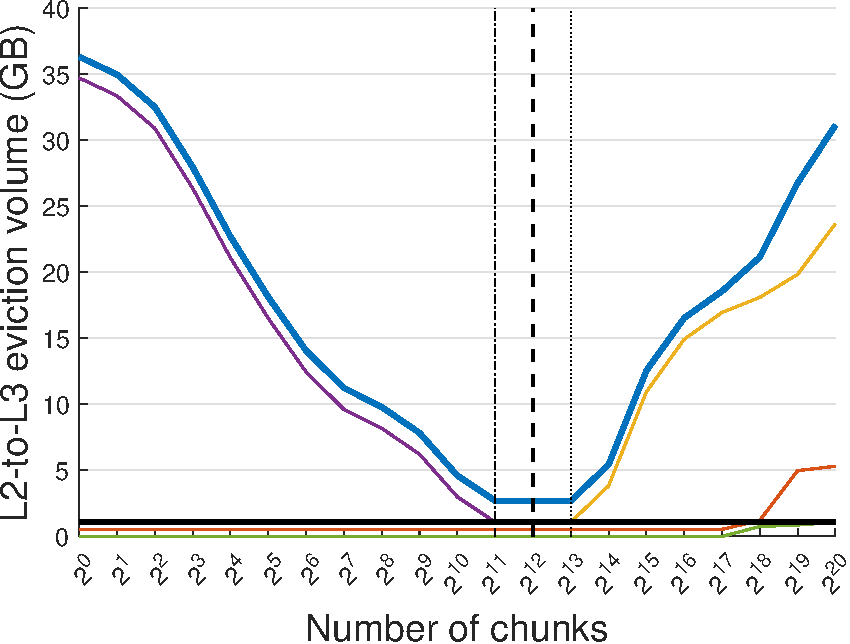
\includegraphics[width=\figwidth]{figs/spr_buildingBlocks_varyChunks_scale29_L3Evict.pdf}
\end{tabular}
\caption{Wall-clock time (top) and L2-to-L3 cache evictions (bottom) versus the number of chunks for a set of microbenchmarks that test the performance of the building blocks of MAGNUS.
A single core of the SPR system is used (see \autoref{tab:machines}). \textit{Total} denotes the sum of the building block times, and \textit{Stream} is a standard streaming benchmark that serves as the peak-performance baseline. The middle vertical dashed line denotes the optimal number of fine-level chunks.
The left and right dashed lines denote the point at which the storage requirement of the reorder and dense accumulation arrays exceed the L2 cache size, respectively.}
\label{fig:building_blocks_varyChunks}
\end{figure}

\subsubsection{Building Blocks of MAGNUS}
In this experiment, MAGNUS is deconstructed into its building blocks: histogramming, prefix summing, reordering, and accumulation.
For the algorithmic details of each building block, see the associated comments in \autoref{alg:magnus_fine} and \autoref{alg:magnus_coarse}. For example, the algorithm for histogramming is on lines 3-6 in \autoref{alg:magnus_fine} and lines 3-10 in \autoref{alg:magnus_coarse}.
\autoref{fig:building_blocks_varyChunks} shows time and the volume of L2-to-L3 cache evictions (measured using Likwid~\cite{likwid}) versus the number of chunks for a stream size and length of $2^{29}$ elements.
This stream length results in the size of the dense accumulation array varying from $2^{29}$ to $2^{29}/2^{20} = 512$ as the number of chunks increases.
This emulates the per-chunk dense accumulation in MAGNUS.
The time for a standard streaming benchmark is shown, which consists of performing contiguous reads from the input arrays and contiguous writes to the output arrays.
This serves as our peak performance baseline, where the total time (i.e., the sum of all the building block times) cannot exceed the streaming time.
The left and right dashed lines are the points at which the reorder and dense accumulation data structures exceed the L2 cache size.
The middle vertical dashed line shows the optimal number of fine-level chunks (derived in \autoref{sec:magnus_opt_params}), which is calculated using the stream length in place of $m_C$ in \autoref{equ:fine_level_nchunks_optimal}.

The total time, which closely approximates the performance of the fine-level algorithm, is dominated by dense accumulation and reordering.
The time for reordering increases significantly past $2^{13}$, where the storage requirement (active cache lines, histogram array, and prefix sum array) exceeds the L2 cache size, as seen by the increase in L2-to-L3 cache evictions.
For dense accumulation, performance improves as the number of chunks increases due to the reduced size of the dense accumulation array; this is a key result of our locality generation approach.
The total execution time reaches a minimum at the optimal number of fine-level chunks, where both dense accumulation and reordering achieve optimal cache behavior. At this point, the total time is $\approx 2.2$ times the streaming time. Although lower-level optimizations, such as vectorized histogramming, could further decrease this slowdown, maintaining this reasonably small multiple of the peak performance is crucial for scaling to massive matrices.
We will show in \autoref{sec:results_spgemm} that MAGNUS can maintain a similar multiple of the peak performance for massive random matrices, while other SpGEMM baselines cannot.

\autoref{fig:building_blocks_varyMaxIdx} illustrates the impact of varying the stream length, where the optimal number of fine-level chunks is chosen for each value of the stream length.
Past a stream length of $2^{31}$, the total time rises sharply due to the high volume of L2-to-L3 cache evictions.
This behavior highlights the necessity of the coarse-level algorithm in MAGNUS: even when the optimal number of fine-level chunks is used, the total storage cost of all data structures can exceed the L2 cache capacity when the number of columns of $C$ is sufficiently large.
In MAGNUS, the coarse-level algorithm automatically activates after the breaking point at $2^{31}$.
Consequently, each coarse-level chunk contains column indices in the range $[0, 2^{31})$, allowing the fine-level data structures to fit into the L2 cache.
The fine-level algorithm is then applied to each coarse-level chunk and is cache-efficient.


\begin{figure}[t]
\centering
\begin{tabular}{c}
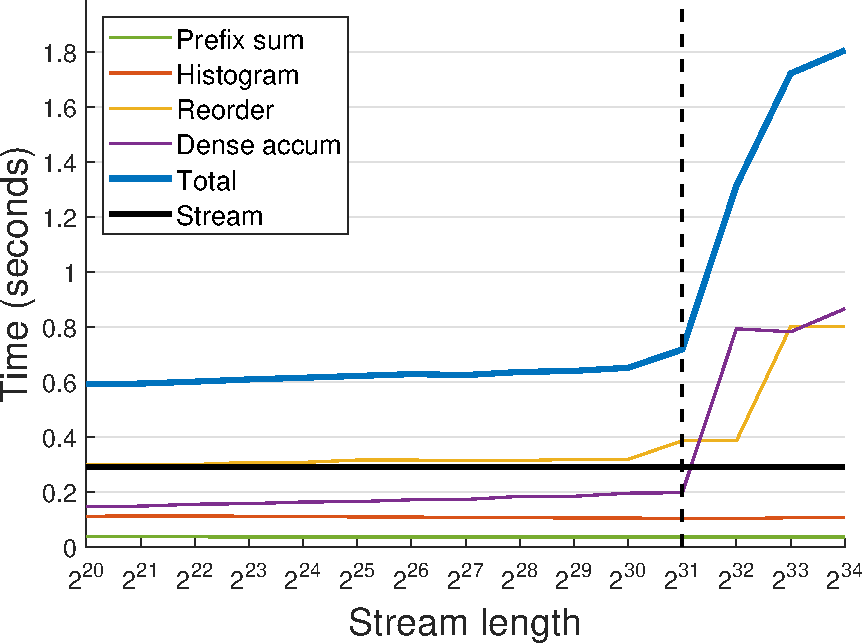
\includegraphics[width=\figwidth]{figs/spr_buildingBlocks_varyMaxIdx_time.pdf} \\
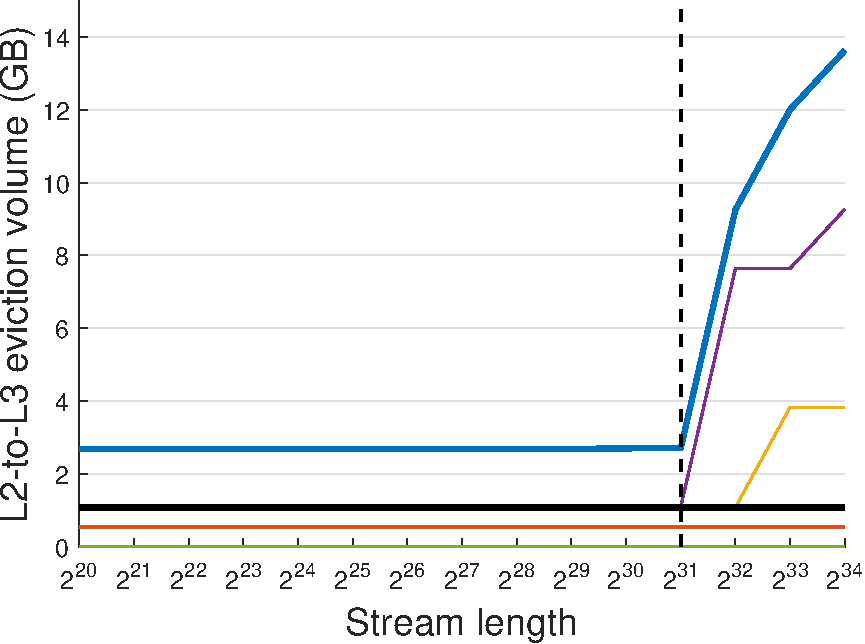
\includegraphics[width=\figwidth]{figs/spr_buildingBlocks_varyMaxIdx_L3Evict.pdf}
\end{tabular}
\caption{Wall-clock time (top) and L2-to-L3 cache evictions (bottom) versus the stream length of the input stream for a set of microbenchmarks that test the performance of the building blocks of MAGNUS.  For each stream length value, the optimal number of fine-level chunks is chosen (see \autoref{sec:magnus_opt_params}). \textit{Total} denotes the sum of the building block times, and \textit{Stream} is a standard streaming benchmark that serves as the peak-performance baseline.
The vertical dashed line denotes the threshold at which the fine-level data structures exceed the L2 cache capacity.}
\label{fig:building_blocks_varyMaxIdx}
\end{figure}

In summary, our microbenchmarks give us two key conclusions.
First, when both the stream length and size are large, neither sort-based nor dense accumulation performs optimally. However, the relatively inexpensive reordering mechanism in MAGNUS effectively mitigates these issues by reducing both of these quantities. For chunks with a small number of elements, sorting can be applied. Otherwise, dense accumulation is more efficient due to the short stream length per chunk, which allows the accumulation data structures to fit in the L2 cache.

Second, our microbenchmarks provide insight into the overall performance of the coarse- and fine-level algorithms.
The reordering microbenchmark closely approximates the coarse-level algorithm since the dominant cost of the coarse-level algorithm is its reordering phase.
Therefore, the coarse-level algorithm is approximated to perform at near-streaming speed up to the breaking point of $2^{13}$ chunks.
For realistic matrices, this breaking point is likely not reached since that would require the multiplication of matrices with more than $2^{31}2^{13} = 2^{44}$ columns.
The performance of the fine-level algorithm is closely approximated by \textit{Total}, which is dominated by the time for reordering and dense accumulation.
The significant decline in the performance of \textit{Total} beyond a stream length of $2^{31}$ underscores the importance of the initial, near-streaming-speed pass over the intermediate product provided by the coarse-level algorithm.
Rather than using the fine-level algorithm beyond this $2^{31}$ threshold, a comparatively inexpensive initial reordering step yields better performance.
Note that these thresholds ($2^{13}$ and $2^{31}$) are system-dependent; MAGNUS automatically calculates these thresholds using the input system parameters (see \autoref{sec:magnus_opt_params}).


\subsection{Test Configuration for SpGEMM}
\begin{figure*}[!htbp]
\centering
\begin{tabular}{m{0.03\linewidth} m{0.97\linewidth}}
\textbf{EMR} &
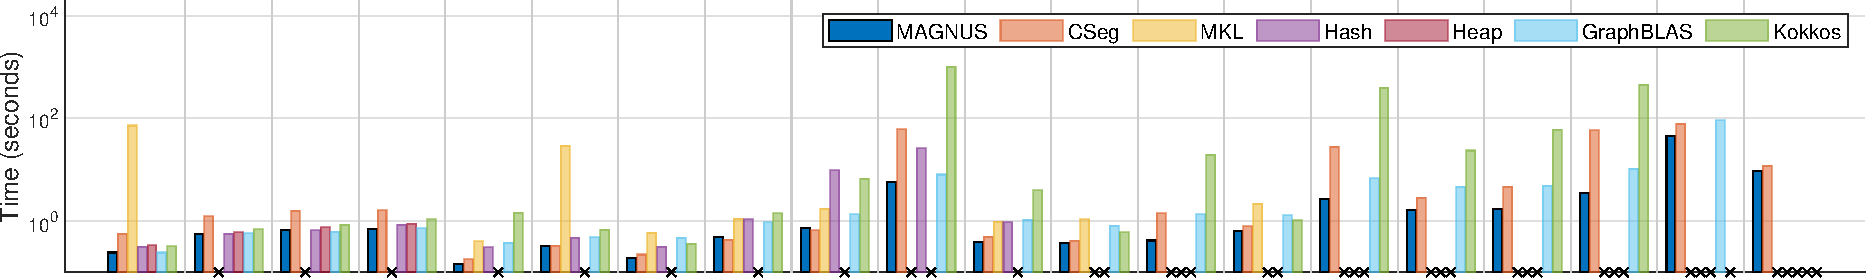
\includegraphics[width=0.96\linewidth]{figs/baselines_emr_SuiteSparse_time_bars.pdf} \\
\textbf{SPR} &
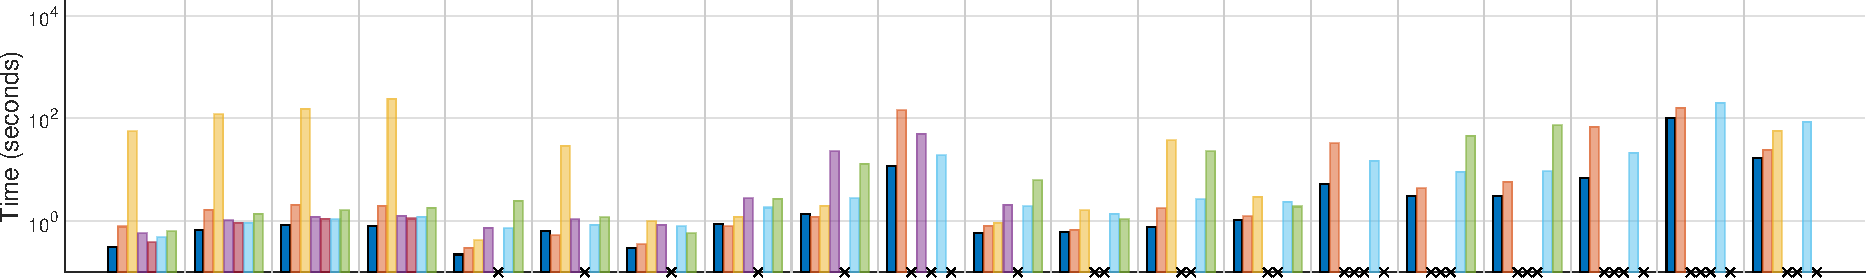
\includegraphics[width=0.96\linewidth]{figs/baselines_spr_SuiteSparse_time_bars.pdf} \\
\raisebox{2.5em}{\textbf{SKX}} &
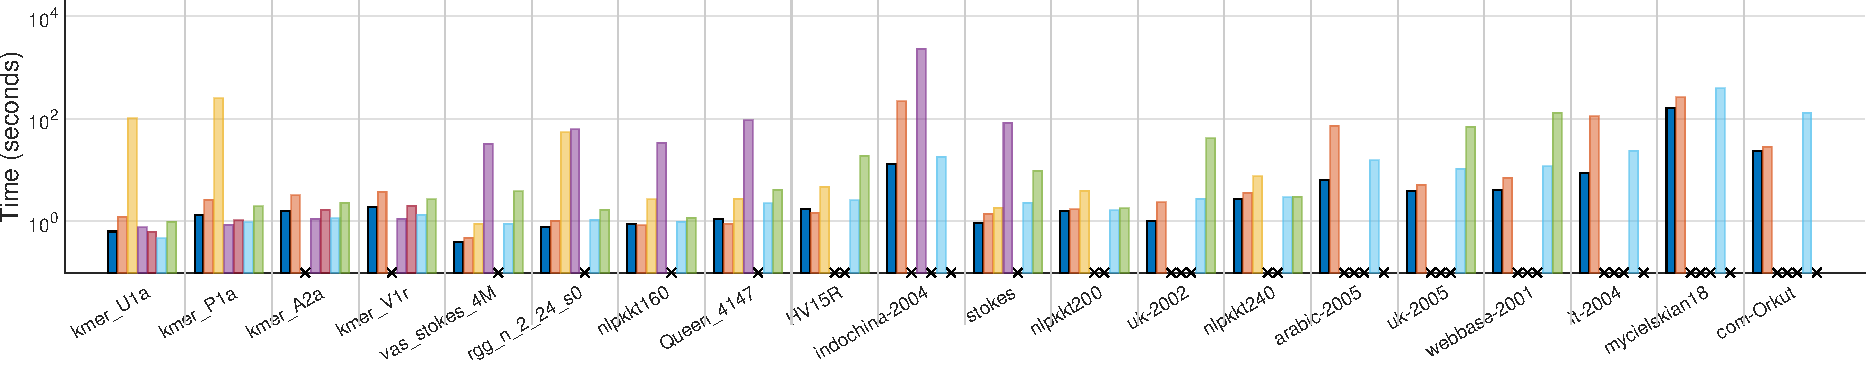
\includegraphics[width=0.96\linewidth]{figs/baselines_skx_SuiteSparse_time_bars.pdf} \\
\end{tabular}
\caption{Wall-clock time in log scale for the SuiteSparse matrix collection.
The $\times$-shaped markers denote failed runs (out-of-memory or segmentation faults) of the baselines.
All available threads were used for each system.}
\label{fig:baselines_suitesparse}
\end{figure*}

In the next section, we compare an OpenMP implementation of MAGNUS to a diverse set of state-of-the-art baselines:
CSeg~\cite{cseg}, Intel MKL~\cite{mkl}, vectorized hash/heap-based algorithms~\cite{nagasaka1,nagasaka2}, SuiteSparse:GraphBLAS~\cite{graphblas}, and Kokkos~\cite{kokkos,kokkos2}.
For MKL, we use the sparse BLAS inspector-executor API, i.e., the function \texttt{mkl\_sparse\_spmm()}.
CSeg is the only baseline that implements a locality-generation algorithm, and to the best of our knowledge, it is the only algorithm other than MAGNUS that does so.

We report the total SpGEMM time for all algorithms, where the total time is the sum of the pre-processing, symbolic, numeric, and post-processing phases.
For example, the total time for CSeg is the sum of the time taken to construct the high-level summary matrix and perform the symbolic and numeric phases.  
In contrast, for MKL, we measure only the time of the call to \texttt{mkl\_sparse\_spmm()}, as that is the only operation exposed to us.
For MAGNUS, the total time is the sum of the setup, symbolic, and numeric phases.
We perform one warm-up run and then extract the time by taking the average of the next 10 runs.
We found that the time did not vary significantly between many runs.
Our test systems are shown in \autoref{tab:machines}, all of which use Intel processors.
We utilized all available threads, including hyperthreads, for all SpGEMM runs, resulting in the fastest execution time for both the baseline implementations and MAGNUS.

\begin{table}[htbp]
\caption{Hardware specifications of the test systems.
All systems are a single multisocket node with Intel CPUs.}
\begin{center}
\resizebox{\columnwidth}{!}{
\begin{tabular}{lrrr}
\hline
Architecture & Skylake (SKX) & Sapphire Rapids (SPR) & Emerald Rapids (EMR) \\
\hline
Xeon Model & Gold 6140 & Gold 6438M & Platinum 8592+ \\
%GHz & 2.3 & 2.2 & 1.9 \\
Sockets & 4 & 2 & 2 \\
Total cores and threads & 72 and 144 & 64 and 128 & 128 and 256 \\
L1 size per core & 32 KB & 48 KB & 48 KB \\
L2 size per core & 1 MB & 2 MB & 2 MB \\
L3 size per socket & 24.75 MB & 60 MB & 320 MB \\
Memory & 2 TB & 4 TB & 1 TB \\
\hline
\end{tabular}
}
\label{tab:machines}
\end{center}
\end{table}

\begin{table}[htbp]
\caption{Properties of the SuiteSparse matrices.}
\begin{center}
\resizebox{\columnwidth}{!}{
\begin{tabular}{lrrrrr}
\hline
Matrix & $n_A$ & $nnz_A$ & $nnz_{A^2}/n_{A^2}$ & $nnz_{A^2}$ \\
\hline
kmer\_U1a & 67,716,231 & 138,778,562 & 3.3 & 222,262,359 \\
kmer\_P1a & 139,353,211 & 297,829,984 & 3.8 & 531,367,449 \\
kmer\_A2a & 170,728,175 & 360,585,172 & 3.6 & 622,660,207 \\
kmer\_V1r & 214,005,017 & 465,410,904 & 3.9 & 824,450,881 \\
vas\_stokes\_4M & 4,382,246 & 131,577,616 & 188.6 & 826,486,449 \\
rgg\_n\_2\_24\_s0 & 16,777,216 & 265,114,400 & 49.4 & 828,639,073 \\
nlpkkt160 & 8,345,600 & 229,518,112 & 148.7 & 1,241,294,184 \\
Queen\_4147 & 4,147,110 & 329,499,284 & 362.2 & 1,501,950,816 \\
HV15R & 2,017,169 & 283,073,458 & 876.5 & 1,768,066,720 \\
indochina-2004 & 7,414,866 & 194,109,311 & 263.3 & 1,952,630,542 \\
stokes & 11,449,533 & 349,321,980 & 184.7 & 2,115,146,825 \\
nlpkkt200 & 16,240,000 & 448,225,632 & 149.4 & 2,425,937,704 \\
uk-2002 & 18,520,486 & 298,113,762 & 172.5 & 3,194,986,138 \\
nlpkkt240 & 27,993,600 & 774,472,352 & 149.8 & 4,193,781,224 \\
arabic-2005 & 22,744,080 & 639,999,458 & 366.0 & 8,323,612,632 \\
uk-2005 & 39,459,925 & 936,364,282 & 227.4 & 8,972,400,198 \\
webbase-2001 & 118,142,155 & 1,019,903,190 & 114.0 & 13,466,717,166 \\
it-2004 & 41,291,594 & 1,150,725,436 & 340.2 & 14,045,664,641 \\
mycielskian18 & 196,607 & 300,933,832 & 195,076.4 & 38,353,378,617 \\
com-Orkut & 3,072,441 & 234,370,166 & 16,220.6 & 49,836,711,933 \\
\hline
\end{tabular}
}
\label{tab:suite_sparse}
\end{center}
\end{table}

\begin{table}[htbp]
\caption{Properties of the RMat16 matrices (R-mats with an average of 16 nonzero entries per row).
The standard Graph500 parameters are used ($a = .57$ and $b = c = .19$).}
\begin{center}
\resizebox{\columnwidth}{!}{
\begin{tabular}{lrrrrr}
\hline
Scale & $n_A$ & $nnz_A$ & $nnz_{A^2}/n_{A^2}$ & $nnz_{A^2}$ \\
\hline
18 & 262,144 & 4,194,304 & 5,141.7 & 1,347,858,618 \\
19 & 524,288 & 8,388,608 & 7,072.6 & 3,708,083,907 \\
20 & 1,048,576 & 16,777,216 & 9,479.9 & 9,940,402,266 \\
21 & 2,097,152 & 33,554,432 & 12,377.9 & 25,958,392,028 \\
22 & 4,194,304 & 67,108,864 & 16,387.1 & 68,732,382,095 \\
23 & 8,388,608 & 134,217,728 & 22,253.2 & 186,673,674,064 \\
\hline
\end{tabular}
}
\label{tab:rmat16_stats}
\end{center}
\end{table}

We consider three important matrix test sets: matrices from the SuiteSparse collection~\cite{suitesparse}, recursive model power-law matrices (R-mats)~\cite{rmat}, and uniform random matrices (i.e., those from the Erd\H{o}s--R\'enyi (ER) model)~\cite{erdosrenyi}.
For the SuiteSparse and R-mat test sets, we consider the operation $A^2$ for square $A$, which is the de facto standard for evaluating SpGEMM algorithms.
The configuration for the uniform random matrix set will be discussed later in this section.
\autoref{tab:suite_sparse} shows the set of SuiteSparse matrices used in our experiments, where $nnz_{A^2}/n_{A^2}$ is the average number of nonzero entries per row of $A^2$, which is a measure of the sparsity of $A^2$.
These matrices are the largest 20 (in terms of the total number of nonzero entries in $A$) in which both the $A$ and $A^2$ (the result of SpGEMM in our experiments) fit into memory for MAGNUS and at least one baseline.
\autoref{tab:rmat16_stats} shows the R-mats with an average of 16 nonzero entries per row, where the table is organized by increasing \emph{scale}, e.g., the scale-18 R-mat has $2^{18}$ rows.
The standard Graph500 parameters were used to generate these R-mats ($a = .57$ and $b = c = .19$).
The scale-23 matrix is the largest in which both the input
and output fit into memory for MAGNUS and at least one baseline on the SPR system.

\subsection{SpGEMM Results}\label{sec:results_spgemm}

\begin{figure}[htbp]
\newcommand{\figwidthLoc}{.95\linewidth}
\centering
\begin{tabular}{c}
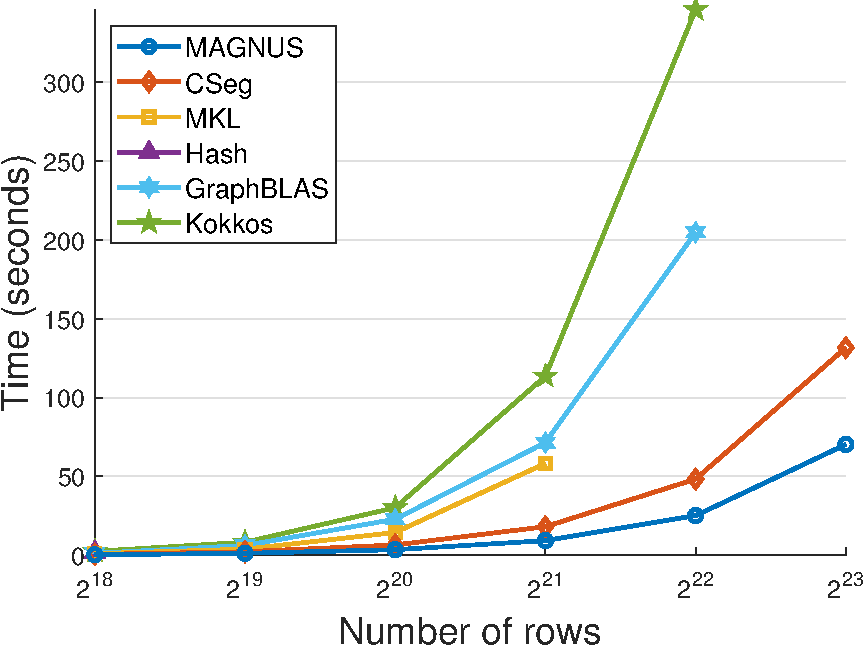
\includegraphics[width=\figwidth]{figs/baselines_spr_rmat16_time.pdf} \\
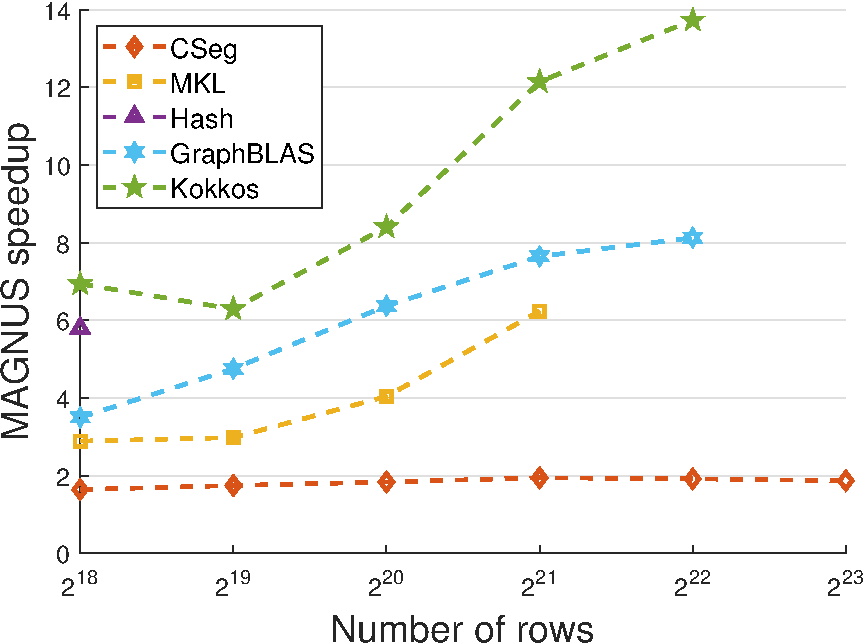
\includegraphics[width=\figwidth]{figs/baselines_spr_rmat16_speedup.pdf}
\end{tabular}
\caption{Wall-clock time and speedup versus number of rows for the RMat16 matrix set on the SPR system (see \autoref{tab:machines}).
The speedup is the ratio of the time of the baselines to that of MAGNUS.}
\label{fig:baselines_rmat16}
\end{figure}

\begin{figure*}[htbp]
\newcommand{\figwidthLoc}{.31\linewidth}
\centering
\begin{tabular}{ccc}
\textbf{EMR} & \textbf{SPR} & \textbf{SKX} \\
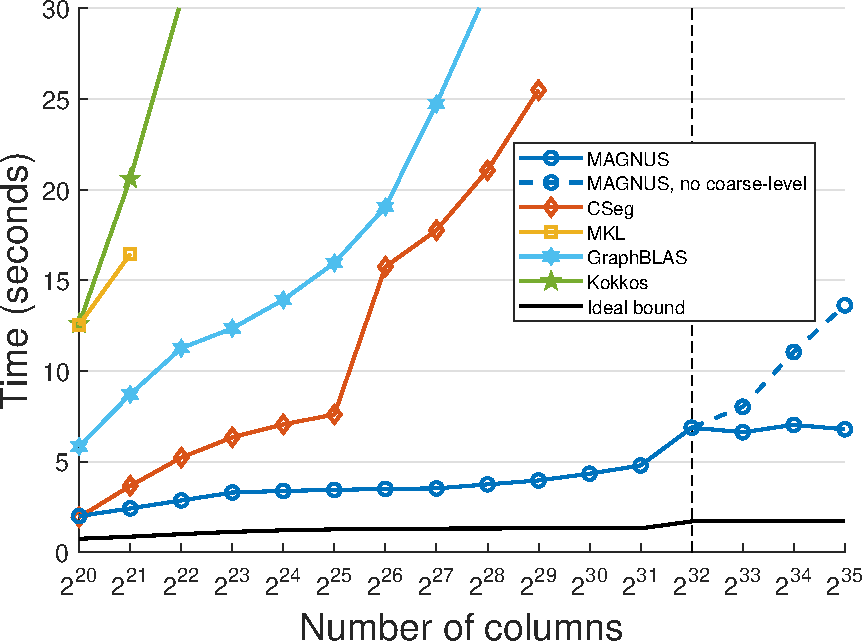
\includegraphics[width=\figwidthLoc]{figs/emr_massiveER_varyScale_nnz2048.pdf} &
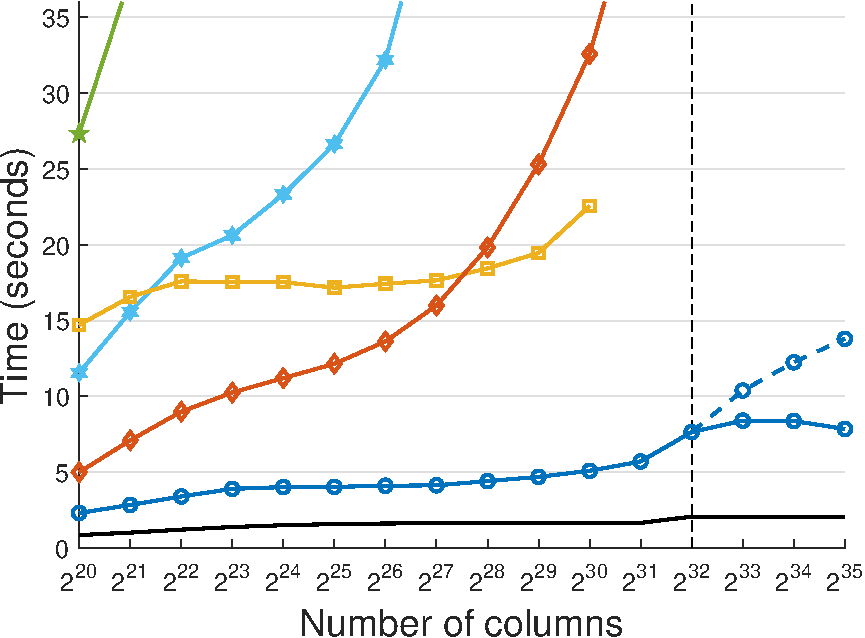
\includegraphics[width=\figwidthLoc]{figs/spr_massiveER_varyScale_nnz2048.pdf} &
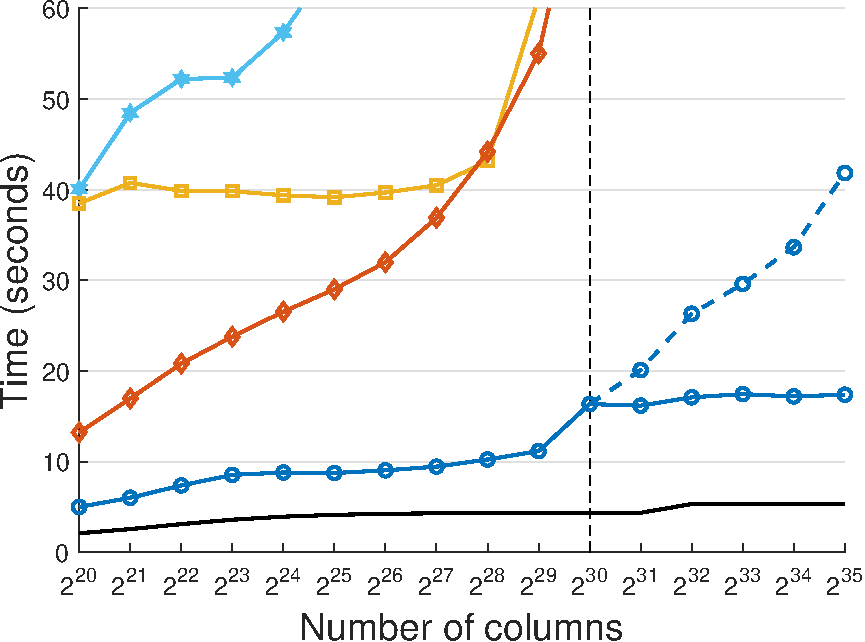
\includegraphics[width=\figwidthLoc]{figs/skx_massiveER_varyScale_nnz2048.pdf}
\end{tabular} 
\caption{Time versus number of columns of $C$ for the uniform random matrix test set.
A fixed average number of nonzero entries per row of 2048 is used.
The vertical dashed line denotes the point at which MAGNUS begins to use the coarse-level algorithm.}
\label{fig:massiveERs_varyScale}
\end{figure*}

We first consider the SuiteSparse matrix collection.
\autoref{fig:baselines_suitesparse} shows the execution time in logarithmic scale for each matrix and each system.
%The speedup is defined as the ratio of the baseline times to that of MAGNUS.
In some cases, out-of-memory errors and segmentation faults caused some of the baselines to fail, denoted by the missing bars.
MAGNUS is often faster than all baselines and is often orders of magnitude faster than at least one baseline.
CSeg is sometimes slightly faster than MAGNUS (up to $1.23\times$) for Queen\_4147, HV15R, rgg\_n\_2\_24\_s0, and nlpkkt160.
For these matrices, MAGNUS places all rows into the dense accumulation category due to their banded structure, i.e., these matrices do not require locality generation to be efficiently multiplied.
This suggests that in the absence of locality generation, the accumulators in CSeg may be slightly more optimized for banded matrices.
Similarly, the kmer matrices also do not require locality generation, where Hash, Heap, and GraphBLAS are slightly faster than MAGNUS in several cases.
These matrices are not banded but are highly sparse, leading to an intermediate product per row that is less than our dense accumulation threshold.
Therefore, sort- or hash map-based accumulators are most effective, as shown by MAGNUS, Hash, and Heap having the fastest times (most rows in MAGNUS are placed into the sort category).

In all other cases, MAGNUS categorizes rows as a mixture of sorting, dense accumulation, and fine-level locality, 
where a significant number of rows require the fine-level algorithm (for all SuiteSparse matrices, the coarse-level algorithm is not needed).
MAGNUS is the fastest method for 76\% of the 60 test cases (20 matrices across three systems) and is always the fastest for the 11 largest matrices.
MAGNUS is up to $16.6$, $306.7$, $172.5$, $1.4$, $5.7$, and $171.8$ times faster than CSeg, MKL, Hash, Heap, GraphBLAS, and Kokkos, respectively, and is only $1.4$ times slower than any of the baselines in the worst case.
The low peak speedup over Heap is due to the high failure rate of Heap, which only ran to completion for the kmer matrices.

\autoref{fig:baselines_rmat16} shows the time and speedup versus the number of rows for the RMat16 matrix set on the SPR system, where the speedup is the ratio of the time of the baselines to that of MAGNUS.
The SPR system, which has the largest memory, allows us to scale to the largest RMat16 matrix.
Showing results for the other two systems does not provide additional insight.
Since we are using the standard Graph500 parameters, a small average number of nonzero entries per row (16 in this case) produces a high amount of fill-in in $C$ (as shown in \autoref{tab:rmat16_stats}) because many of the nonzero entries in $A$ are clustered in the top left corner.
Unlike banded and other highly sparse structures that produce less fill-in and more regular access patterns, the mixture of a random distribution with clustering in the RMat16 matrices is problematic for conventional accumulators since a high data volume across a wide range of column indices results in data structures that do not fit into the L2 cache.
This is demonstrated in \autoref{fig:baselines_rmat16}, which illustrates the poor scaling of all baselines, except for CSeg, as the scale increases.
Heap failed in all cases and Hash failed in all but the smallest case.
MAGNUS is $6.2$, $5.8$, $8.1$, and $13.7$ times faster than MKL, Hash, GraphBLAS, and Kokkos, respectively, for the largest matrices.
The scaling of CSeg and MAGNUS demonstrates the importance of locality generation.
Although MAGNUS is $\approx1.8$ times faster than CSeg, they both scale at a similar rate.


Lastly, we consider uniform random matrices.
Unlike the R-mats, a small number of nonzero entries per row does not produce a high amount of fill-in in $C$. 
However, as we scale up the number of columns and nonzero entries per row of $B$, the uniform distribution of the column indices results in frequent accesses to the entire accumulator.
For conventional accumulators, this becomes cache-inefficient if no locality generation strategy is used.
Since the performance of conventional accumulators is sensitive to the number of columns of $C$ and not to the number of rows (see \autoref{sec:microbench}), we consider the nonsquare case where $C$ has 4096 rows and a variable number of columns.
This allows us to scale to massive matrices without exceeding the memory limit of our systems.
Furthermore, only the rows of $B$ that depend on the nonzero entries in $A$ are generated, saving additional memory.


\autoref{fig:massiveERs_varyScale} shows results for increasing the number of columns with a fixed average number of nonzero entries per row of 2048.
Hash and Heap failed in all cases.
The black line is the ideal performance bound, which is calculated by dividing the minimum required data volume for Gustavson-based SpGEMM by the system bandwidth, i.e., $T_{ideal} = \frac{n_{readVol}+n_{writeVol}}{r_{bw}}$,
where the system bandwidth $r_{bw}$ was measured using a streaming microbenchmark.
The ideal read volume is
\begin{equation}
\begin{aligned}
n_{readVol} = & 2(n_A+1) s_{rowPtr} + nnz_A(4s_{rowPtr} + 2s_{colIdx} + s_{val}) + \\
& n_{interProd} (2s_{colIdx} + s_{val}),
\end{aligned}
\label{equ:ideal_data_vol}
\end{equation}
where $s_{rowPtr}$ is the size of the CSR row pointer type (\texttt{size\_t} in our implementation), $s_{colIdx}$ is the size of the column index type (\texttt{uint32\_t} or \texttt{uint64\_t} depending on the size of the matrix), and $s_{val}$ is the matrix coefficient value type (\texttt{float} in our experiments).
The first term denotes the read volume of the row pointers of $A$; the second term denotes the read volume of the nonzero entries in $A$ and the row pointers in $B$; and the third term, which is the asymptotically dominant term, denotes the read volume of the nonzero entries in the rows of $B$.
The number of elements in the intermediate product is defined as $n_{interProd} = \sum_{(i,j)\in \mathcal{S}(A)}nnz_{B_j}$.
The factors of two account for the symbolic and numeric phases.
The factor of four accounts for the symbolic phase, the numeric phase, and the need to read both the start and end row pointers for each row of $B$ (in contrast to the reading of rows of $A$, the rows of $B$ are read nonconsecutively).

The ideal write volume is 
\begin{equation}
n_{writeVol} = (n_C+1) s_{rowPtr} + nnz_C (s_{colIdx} + s_{val}),
\end{equation}
with the first term corresponding to writing the row pointers of $C$ and the second term to writing the nonzero entries.
The overall data volume is the sum of the read and write data volumes.
This ideal bound does not account for various costs, such as NUMA effects, synchronization overheads, or the performance of accessing intermediate data structures (e.g., the accumulator), which can have a significant impact on the performance of SpGEMM algorithms.
Additionally, this bound does not consider cached rows of $B$, as reflected in the expression for $n_{interProd}$, which assumes that previously read rows of $B$ are not reused.
For this reason, we only consider this bound for the uniform random matrices, where there is minimal opportunity for row reuse in $B$.


\autoref{fig:massiveERs_varyScale} shows that MAGNUS maintains an average multiple of $\approx 2.7$ of the ideal bound before applying the coarse-level algorithm and $\approx 3.5$ afterward.
The increase in the multiple is due to the increase in data volume incurred by the outer product (additionally, the slight increase in the ideal bound at $2^{32}$ is due to a change from \texttt{uint32\_t} to \texttt{uint64\_t} for $s_{colIdx}$).
The $2.7$ multiple is consistent with the multiple from our microbenchmarks.
In contrast, the baselines, including CSeg, diverge from the ideal bound.
This suggests that the locality generation method in CSeg, which explicitly constructs an auxiliary segmented matrix, does not scale if a large number of segments is required.
The vertical dashed line shows the point at which MAGNUS starts to place rows in the coarse-level category.
For SKX, the crossover point occurs at $2^{30}$, compared to $2^{32}$ for SPR and EMR, due to the smaller L2 cache size in SKX.
The dashed blue line shows MAGNUS with the coarse-level algorithm turned off, where MAGNUS diverges from the ideal bound.
This shows the necessity of multiple levels of locality, especially for massive matrices where the fine-level data structures do not fit into the L2 cache.